\chapter{Security Assessment 19.05.2022}
To hold the security assessment up to date and test our application regularly for potential threats we repeat the security assessment again. This assessment is performed on the current project state of our KubeWatch application.

\section{Methodology}
To perform this assessment I combine the vulnerability assessment in form of the threat model some chapters before and the penetration testing with the attempt to exploit the most common vulnerabilities in this assessment. 
This assessment is not that deapth because of the knowledge and the actual project state which is not fully finished yet and so this assessment is just a regularly check if all the common OWASP Top 10 are mitigated. For more detail about the security test concept you will find a detailed list in the test concept chapter.

To perform this assessment the following Tools are used: Browser, Nikto, Burp Proxy

\section{Scope}
This security assessment is security a test for our KubeWatch application. The security will be tested on the production environment which is located in the INS Cluster.
The goal of the assessment is to check the KubeWatch application for common vulnerabilities. This assessment will only cover the most common vulnerabilities from the threat model and is not a final security assessment.

\section{Report Summary}
As of commit \lstinline "395938f7" from 19 May 2022, we did not find any known vulnerabilities in the KubeWatch application by testing only the OWASP TOP 10 from the test concept which are relevant for our project. The injection and SSRF attack was unsuccessful.

By testing the KubeWatch application with an additional tampering attack, it will be successful. So Man-in-the-Middle (MITM) is already a problem for our application but with the aspect that this application is only needed for company internal monitoring, the attacker must be already in the system to make a MITM attack successfully with the assumption that the applicattion is only available from the internal network. 

The other analysis with Nikto returns some bad points. Our application need some additional web headers to make it more secure. At the other hand there are some vulnerabilitiey which can possible end up in a insecure direct object reference (IDOR) attack. To prevent this attack we need to check that only routes are available which are needed and return an error if another URL is used.

\section{Detailed Report}

\subsection{Nikto}
\subsubsection{Brief Description}
The first step of this report is to analyse the KubeWatch web application with a common vulnerability analyse tool which is calles Nikto. This tool will check a few things like header options, IDOR attack possibilities for common IDOR attacks.

\subsubsection{Attack}
For this attack i used the described Nikto tool and enter the following command: \newline
\lstinline "nikto -h http://10.20.1.30"

This will test the application by enter a host address.

\subsubsection{Result}
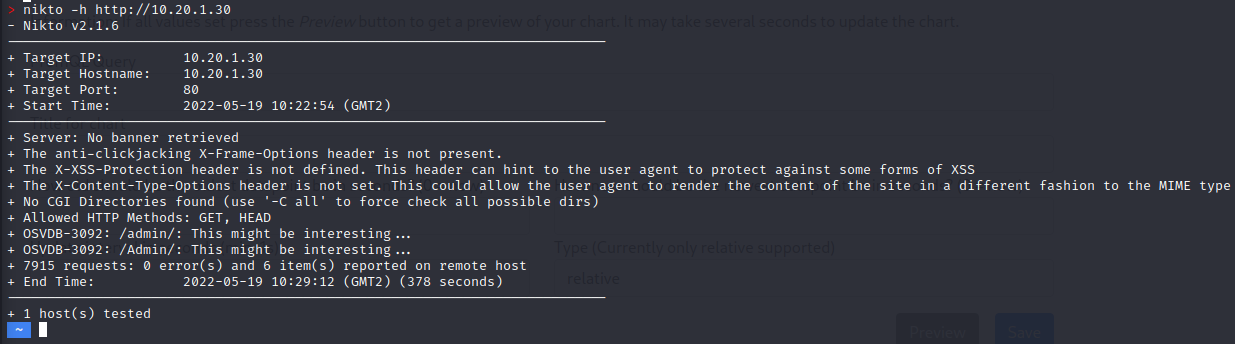
\includegraphics[height=4.15cm]{resources/security_assessment_2_nikto.png} \newline
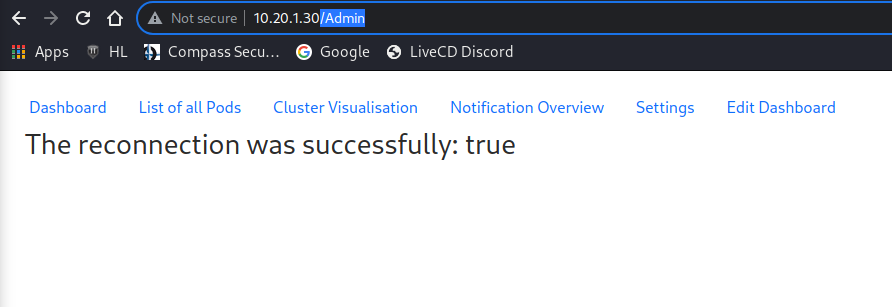
\includegraphics[height=5.15cm]{resources/IDOR-attack.png} \newline

In the screenshot above there are some possible behaviour and header options listed that should be changed to be secure and avoid unexpected behaviour. The following header options should be set in the application:
\begin{itemize}
    \item \lstinline "anti-clickjacking X-Frame-Options"
    \item \lstinline "X-XSS-Protection"
    \item \lstinline "X-Content-Type-Options"
\end{itemize}
The \lstinline "anti-clickjacking X-Frame-Options" header prevents an clickjacking attack on server-side which is described in more detail here: \href{https://owasp.org/www-community/attacks/Clickjacking}{OWASP - Clickjacking}.

The \lstinline "X-XSS-Protection" header mitigate reflected Cross-Site Scripting (XSS) attacks which is described in more detail here: \href{https://developer.mozilla.org/en-US/docs/Web/HTTP/Headers/X-XSS-Protection}{Mozilla - X-XSS-Protection}.

The \lstinline "X-Content-Type-Options" header to avoid MIME type sniffing and is described in more detail here: \href{https://docs.w3cub.com/http/headers/x-content-type-options}{w3cub - X-Content-Type-Options}.

Additionally the routes \lstinline "/admin" and \lstinline "/Admin" should be deleted, because both of them are not needed and they can maybe used as vulnerability.

\subsection{Tampering attack}
\subsubsection{Brief Description}
Tampering attacks allows an attacker to modify the packages between client and server. With this attack a malicious user can exploit the application for own benefits and Man-in-the-Middle (MITM) attack is also one part of tampering.

\subsubsection{Attack}
For this attack I used the Burp Procy tool which allow me to intercept a request and modify it. I tried the attack by adding a new chart to the dashboard.

First I enter a valid PromQL query because I need a reference chart which is valid and withour any tampering attack. \newline
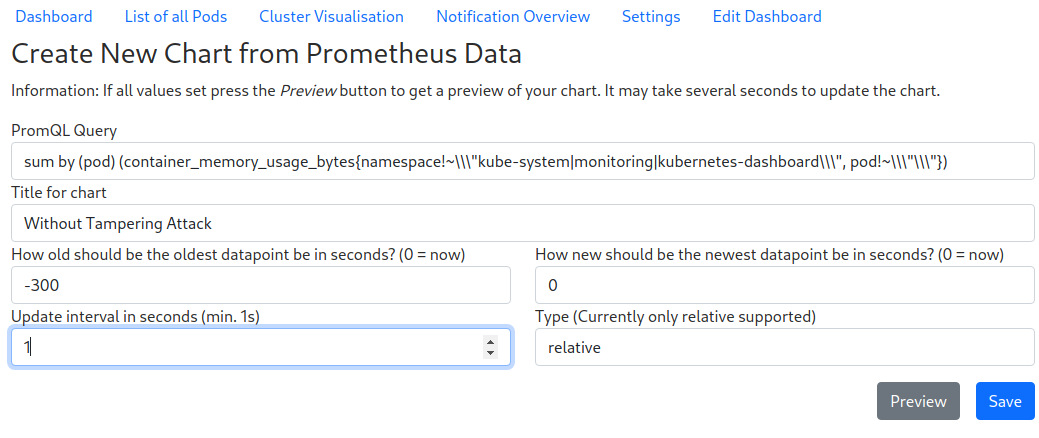
\includegraphics[height=6.5cm]{resources/tampering-without-attack.png}

And then I entered another chart which I stop with the Burp Proxy tool. \newline
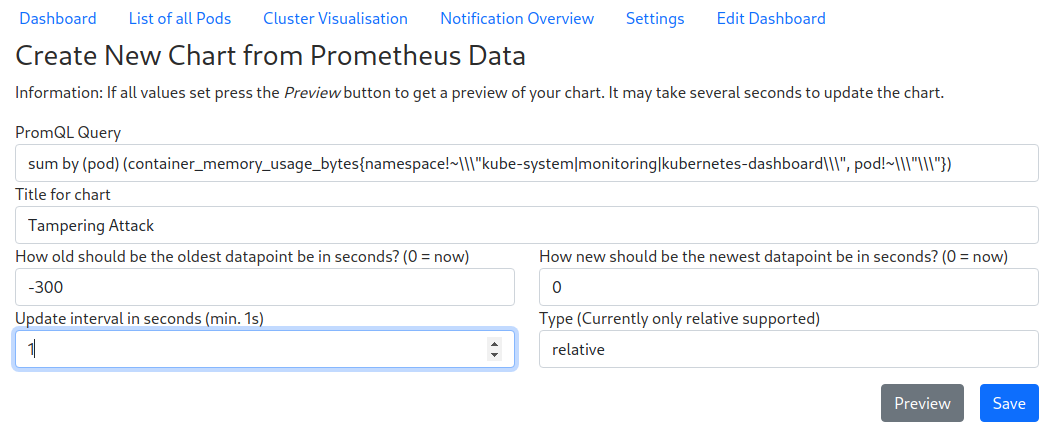
\includegraphics[height=6.5cm]{resources/tampering-attack.png}

In the next step I activate the intercept mode in the Burp Proxy tool to catch the new chart request. There I changed the time period from "-300" to "-500". After that I forward the tampered request and check loading request and response for the dashboard again. \newline
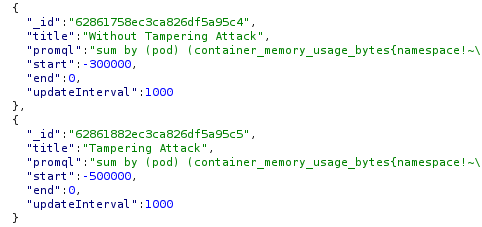
\includegraphics[height=5cm]{resources/tampering-successful-2.png} \newline
Both charts should be the same because I entered both time the same chart input. But you will see the time period is changed now.

\subsection{Injection attack}
\subsubsection{Brief Description}
Injection attacks can occur on two levels in the KubeWatch application: on the KubeWatch Backend API and Prometheus. However, the second is not relevant for this assessment since the only queries are hard-coded and submitted by the backend only.

The KubeWatch Backend API is connected to a MongoDB database which is NoSQL-based. NoSQL injection attacks are possible by using the JSON structure to send queries to the database which are processed as valid commands.

\subsubsection{Attack}
For our assessment, we tried to query the database so that it would return the top-level entry. This can be done by sending the following string via an input field that is supposed to query the database: \lstinline "'{$ne: null}'".

There are currently only one field which take inputs and store them in the MongoDB database. And that is on the \textit{/notifications} page, when you enter a new notifiction.

\subsubsection{Result}
The attack was unsuccessful. This is because of three types of input validation on two different layers.

Firstly, the input forms in the frontend are of type text and type email. This achieves that any input to both fields is treated as text, and additionally, type email requires the specific email format so that no other sequence of characters is allowed. 

Secondly, handlebars are used on the backend which have the benefit when using two curly brackets to retrieve values from a variable, e.g. \lstinline "{{data}}", any value is interpreted as a string. However, if three curly brackets were used, the data input is treated as an object, which would allow execution of e.g. HTML syntax.

Thirdly, since Typescript is used on the backend, the class which is used to store user inputs contains two variables for each input field. Both required the input to be of type string.

These three defence mechanisms thwart any type of injection attack.

\subsection{Server-Side Request Forgery}
\subsubsection{Brief description}
SSRF can currently be attempted on the \textit{/notifications} page, which is temporarily set up to allow the testing of notifications. This page allows two user inputs: one to trigger a test notification, and the second provides a reason to silence the notification.

The triggering of notifications will be disabled in the future, however, the silencing input will remain to allow a user to close any notifications. Since the silencing reason will be stored in the database, there may be injection attacks or even SSRF attacks possible.

\subsubsection{Attack}
Similar to the injection attack, we tried to first trigger the pop-up of an alert using a script: \lstinline "<script>alert('42')</script>". Also, we tried to call a common localhost address, e.g. \lstinline "http://localhost:8080". 

\subsubsection{Result}
Both attempts were unsuccessful. This is again because of input validation on the front- and backend as seen previously in the injection attack.

The frontend input fields allow text only, and the rendering is again performed by handlebars. Both elements are correctly implemented using \lstinline "type=text" and using double curly brackets for the handlebars.

Also, since Typescript is used, the class for handling notifications requires the notification reason and the silencing text to be stored as a string.

All three elements do prevent any successful attempt to either perform an injection or SSRF attack.